\documentclass[oneside,openany,headings=optiontotoc,11pt,numbers=noenddot]{scrreprt}

\usepackage[a4paper]{geometry}
\usepackage[utf8]{inputenc}
\usepackage[T1]{fontenc}
\usepackage{lmodern}
\usepackage[ngerman]{babel}
\usepackage{ngerman}

\usepackage[onehalfspacing]{setspace}

\usepackage{fancyhdr}
\usepackage{fancybox}

\usepackage{rotating}
\usepackage{varwidth}

%Struktogramme
\usepackage[german,curves]{struktex}

\usepackage{pdflscape}
\usepackage{changepage}
\usepackage{graphicx}
\usepackage[bottom]{footmisc}
\usepackage{transparent}
\usepackage{graphbox}
\graphicspath{
	{Pics/PDFs/}
	{Pics/JPGs/}
	{Pics/PNGs/}
}
\usepackage{caption}
\usepackage{wrapfig}
\usepackage{marginnote}
\usepackage{tabularx}
\usepackage{dashrule}
\usepackage{soulutf8}
\usepackage{hhline}
%arydshln suppresses vertical lines in table
%\usepackage{arydshln}
\usepackage{multirow}
\usepackage{enumerate}
\usepackage[hidelinks]{hyperref}
\usepackage{listings}

\usepackage[table]{xcolor}
\usepackage{array}
\usepackage{enumitem,amssymb,amsmath}
\usepackage{interval}
\usepackage{cancel}
\usepackage{stmaryrd}
\usepackage{wasysym}
\usepackage{polynom}
\usepackage{diagbox}
\usepackage{dashrule}
\usepackage{framed}
\usepackage{mdframed}
\usepackage{karnaugh-map}
\usepackage{pdfpages}

\usepackage{blindtext}

\usepackage{eso-pic}

\usepackage{amssymb}
\usepackage{eurosym}

\usepackage[pages=some]{background}
\pagestyle{headings}
\renewcommand{\headrulewidth}{0.2pt}
\renewcommand{\footrulewidth}{0.2pt}
\newcommand*{\underdownarrow}[2]{\ensuremath{\underset{\overset{\Big\downarrow}{#2}}{#1}}}
\setlength{\fboxsep}{5pt}
\newcommand{\explainBelow}[3]{\underbrace{#1}_{\parbox{\widthof{#3}}{\footnotesize\raggedright #2}}}
\newcommand{\explainAbove}[3]{\overbrace{#1}^{\parbox{\widthof{#3}}{\footnotesize\raggedright #2}}}
\newcommand\footnoteref[1]{\protected@xdef\@thefnmark{\ref{#1}}\@footnotemark}


% Codestyle defined
\definecolor{codegreen}{rgb}{0,0.6,0}
\definecolor{codegray}{rgb}{0.5,0.5,0.5}
\definecolor{codepurple}{rgb}{0.58,0,0.82}
\definecolor{backcolour}{rgb}{0.95,0.95,0.92}
\definecolor{deepgreen}{rgb}{0,0.5,0}
\definecolor{darkblue}{rgb}{0,0,0.65}
\definecolor{mauve}{rgb}{0.40, 0.19,0.28}
\colorlet{exceptioncolour}{yellow!50!red}
\colorlet{commandcolour}{blue!60!black}
\colorlet{numpycolour}{blue!60!green}
\colorlet{specmethodcolour}{violet}

%Neue Spaltendefinition
\newcolumntype{L}[1]{>{\raggedright\let\newline\\\arraybackslash\hspace{0pt}}m{#1}}
\newcolumntype{M}{>{\centering\arraybackslash}X}
\newcommand{\cmnt}[1]{\ignorespaces}
%Textausrichtung ändern
\newcommand\tabrotate[1]{\rotatebox{90}{\raggedright#1\hspace{\tabcolsep}}}

%Intervall-Konfig
\intervalconfig {
	soft open fences
}

%Bash
\lstdefinestyle{BashInputStyle}{
	language=bash,
	basicstyle=\small\sffamily,
	backgroundcolor=\color{backcolour},
	columns=fullflexible,
	backgroundcolor=\color{backcolour},
	breaklines=true,
}
%Java
\lstdefinestyle{JavaInputStyle}{
	language=Java,
	backgroundcolor=\color{backcolour},
	aboveskip=1mm,
	belowskip=1mm,
	showstringspaces=false,
	columns=flexible,
	basicstyle={\footnotesize\ttfamily},
	numberstyle={\tiny},
	numbers=none,
	keywordstyle=\color{purple},,
	commentstyle=\color{deepgreen},
	stringstyle=\color{blue},
	emph={out},
	emphstyle=\color{darkblue},
	emph={[2]rand},
	emphstyle=[2]\color{specmethodcolour},
	breaklines=true,
	breakatwhitespace=true,
	tabsize=2,
}
%Python
\lstdefinestyle{PythonInputStyle}{
	language=Python,
	alsoletter={1234567890},
	aboveskip=1ex,
	basicstyle=\footnotesize,
	breaklines=true,
	breakatwhitespace= true,
	backgroundcolor=\color{backcolour},
	commentstyle=\color{red},
	otherkeywords={\ , \}, \{, \&,\|},
	emph={and,break,class,continue,def,yield,del,elif,else,%
		except,exec,finally,for,from,global,if,import,in,%
		lambda,not,or,pass,print,raise,return,try,while,assert},
	emphstyle=\color{exceptioncolour},
	emph={[2]True,False,None,min},
	emphstyle=[2]\color{specmethodcolour},
	emph={[3]object,type,isinstance,copy,deepcopy,zip,enumerate,reversed,list,len,dict,tuple,xrange,append,execfile,real,imag,reduce,str,repr},
	emphstyle=[3]\color{commandcolour},
	emph={[4]ode, fsolve, sqrt, exp, sin, cos, arccos, pi,  array, norm, solve, dot, arange, , isscalar, max, sum, flatten, shape, reshape, find, any, all, abs, plot, linspace, legend, quad, polyval,polyfit, hstack, concatenate,vstack,column_stack,empty,zeros,ones,rand,vander,grid,pcolor,eig,eigs,eigvals,svd,qr,tan,det,logspace,roll,mean,cumsum,cumprod,diff,vectorize,lstsq,cla,eye,xlabel,ylabel,squeeze},
	emphstyle=[4]\color{numpycolour},
	emph={[5]__init__,__add__,__mul__,__div__,__sub__,__call__,__getitem__,__setitem__,__eq__,__ne__,__nonzero__,__rmul__,__radd__,__repr__,__str__,__get__,__truediv__,__pow__,__name__,__future__,__all__},
	emphstyle=[5]\color{specmethodcolour},
	emph={[6]assert,range,yield},
	emphstyle=[6]\color{specmethodcolour}\bfseries,
	emph={[7]Exception,NameError,IndexError,SyntaxError,TypeError,ValueError,OverflowError,ZeroDivisionError,KeyboardInterrupt},
	emphstyle=[7]\color{specmethodcolour}\bfseries,
	emph={[8]taster,send,sendMail,capture,check,noMsg,go,move,switch,humTem,ventilate,buzz},
	emphstyle=[8]\color{blue},
	keywordstyle=\color{blue}\bfseries,
	rulecolor=\color{black!40},
	showstringspaces=false,
	stringstyle=\color{deepgreen}
}

\lstset{literate=%
	{Ö}{{\"O}}1
	{Ä}{{\"A}}1
	{Ü}{{\"U}}1
	{ß}{{\ss}}1
	{ü}{{\"u}}1
	{ä}{{\"a}}1
	{ö}{{\"o}}1
}

% Neue Klassenarbeits-Umgebung
\newenvironment{worksheet}[3]
% Begin-Bereich
{
	\newpage
	\sffamily
	\setcounter{page}{1}
	\ClearShipoutPicture
	\AddToShipoutPicture{
		\put(55,761){{
				\mbox{\parbox{385\unitlength}{\tiny \color{codegray}BBS I Mainz, #1 \newline #2
						\newline #3
					}
				}
			}
		}
		\put(455,761){{
				\mbox{\hspace{0.3cm}
\includegraphics[width=0.2\textwidth]{../../logo.pdf}}
			}
		}
	}
}
% End-Bereich
{
	\clearpage
	\ClearShipoutPicture
}

\geometry{left=2.50cm,right=2.50cm,top=3.00cm,bottom=1.00cm,includeheadfoot}

\begin{document}
	\begin{worksheet}{BGY 16}{Klassenstufe 13 - Mathematik}{Lernabschnitt 1: Kettenregel und Produktregel}
				
		\noindent
		\sffamily
		\begin{framed}
			\noindent
			\small{\color{codegray}\underline{S. 196 \textbf{Aufgabe 2}:}} Berechnen Sie für die natürliche Exponentialfunktion an den Stellen \(-2,\ 0\ \text{und}\ 2\) die Funktionswerte und die Ableitungen. Skizzieren Sie damit den Graphen der Funktion\\
			\par\noindent
			\begin{tabularx}{\textwidth}{M|M|M|M}
				\multicolumn{2}{l}{\(f(x) = e^x\)} & \multicolumn{2}{l}{\(f'(x) = e^x\)}\\
				& & & \\
				x & \(-2\) & \(0\) & \(2\)\\
				\hline
				& & & \\
				\(f(x)\) & \(0,14\) & \(1\) & \(7,39\)\\
				\hline
				& & & \\
				\(f'(x)\) & \(0,14\) & \(1\) & \(7,39\)\\
			\end{tabularx}\\
			\par\bigskip\noindent
			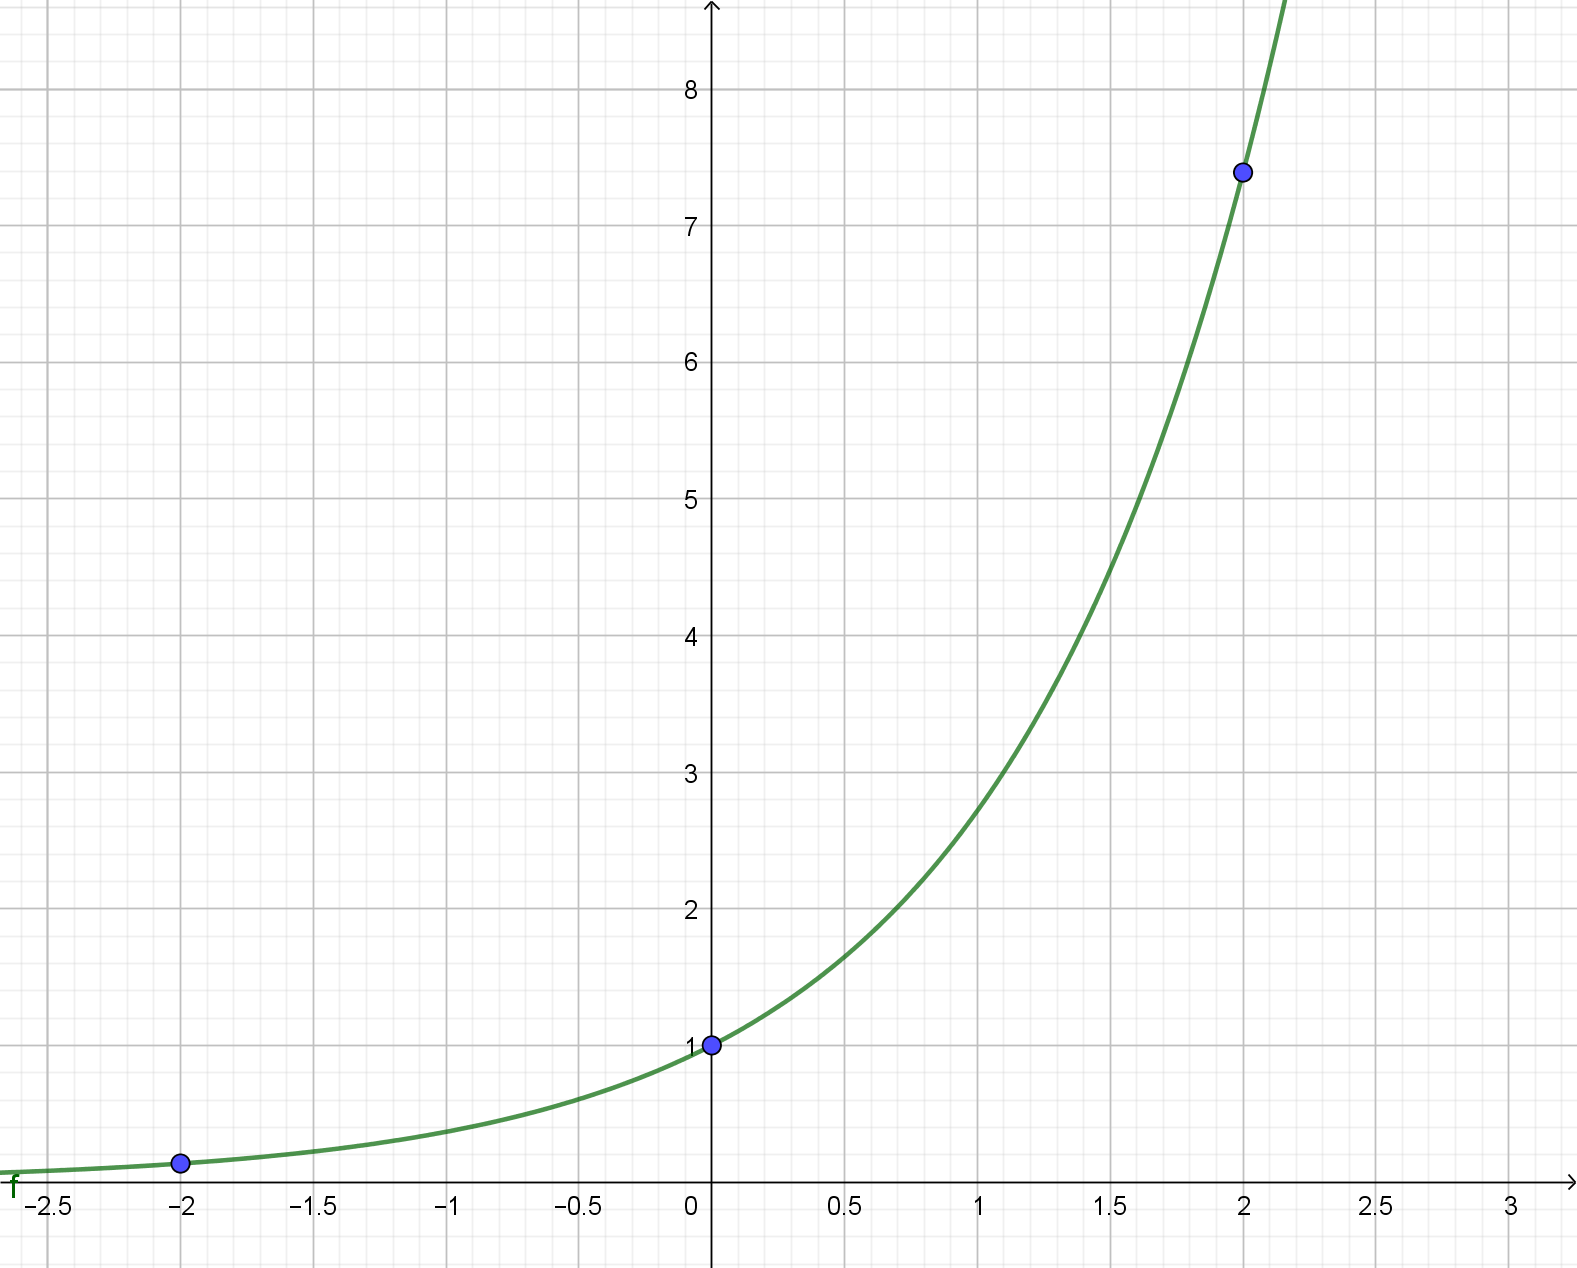
\includegraphics[width=\textwidth]{../99_Bilder/01_ExpFkt/20180921-2.png}
		\end{framed}
		\newpage
		\begin{framed}
			\noindent
			\small{\color{codegray}\underline{S. 196 \textbf{Aufgabe 3}:}} Zeichnen Sie zunächst den Graphen der natürlichen Exponentialfunktion f mit \(f(x) = e^x\). Skizzieren Sie damit den Graphen von\\
			\par\noindent
			\begin{tabularx}{\textwidth}{MMM}
				(a) \(f_1\ \text{mit}\ f_1(x)=e^x+1\) & (a) \(f_2\ \text{mit}\ f_2(x)=2e^x\) & (a) \(f_3\ \text{mit}\ f_3(x)=e^{x-1}\)
			\end{tabularx}\\
			\par\noindent
			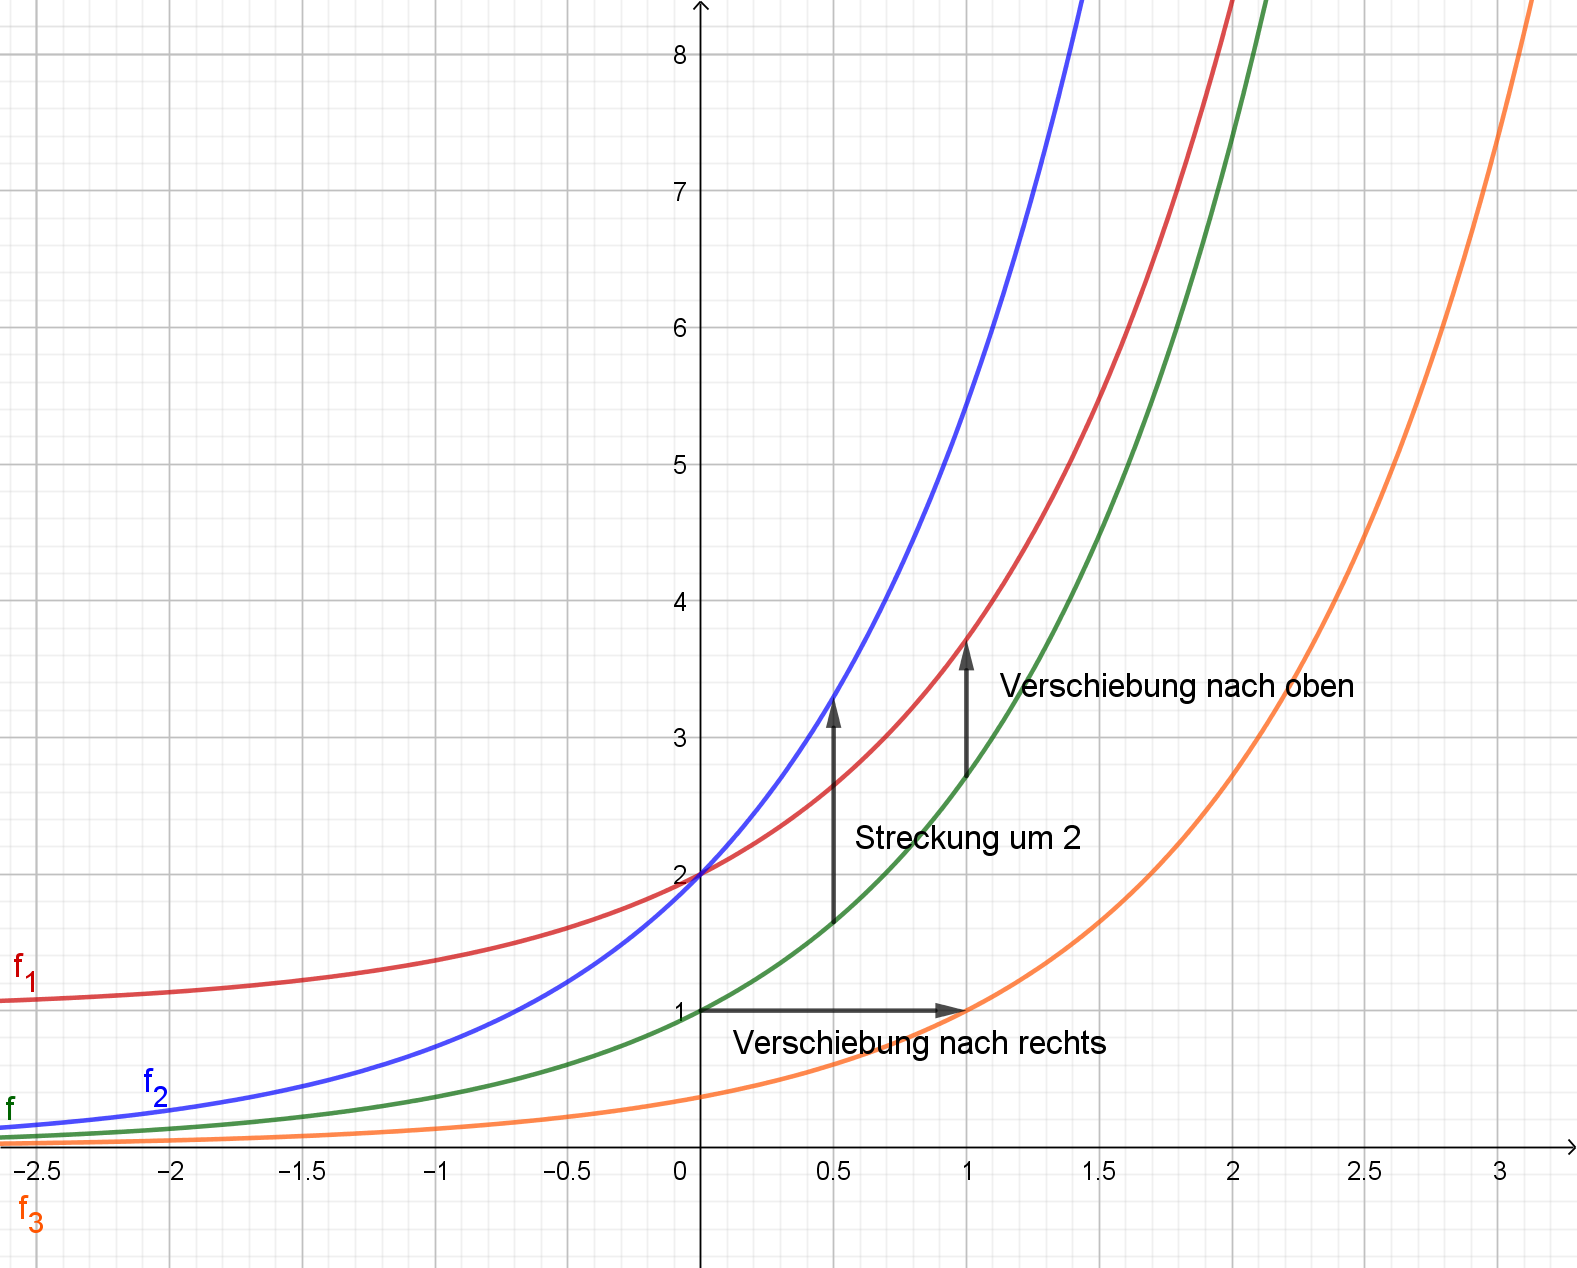
\includegraphics[width=\textwidth]{../99_Bilder/01_ExpFkt/20180921-3.png}
		\end{framed}
		\begin{framed}
			\noindent
			\small{\color{codegray}\underline{S. 196 \textbf{Aufgabe 4}:}} Gegeben ist der Graph K der natürlichen Exponentialfunktion.\\
			\par\noindent
			(a) Bestimmen Sie die Gleichung der Tangenten an K im Punkt \(A(1|e)\) und \(B(-1|\frac{1}{e}\).\\
			(b) Berechnen Sie den Schnittpunkt der Tangente an K im Punkt A mit der x-Achse.
			\begin{framed}
				\noindent
				Wir erinern uns daran, dass die Tangente eine \textit{lineare Funktion} ist. Das bedeutet die Funktion erfüllt folgende Form: \(t(x) = mx+b\).\\
				Dabei entspricht \(\mathbf{m}\) der \textbf{Steigung} der Tangente und \(\mathbf{b}\) gibt den y-Achsenabschnitt der Tangente an.
			\end{framed}
		 	\newpage
		 	\noindent
			(a) Wir beginnen mit der Tangente \(t_A(x)\) an K durch den Punkt \(A(1|e)\).\\
			Hierfür berechnen wir zunächst die Steigung (\(f'(x_p)\)) im geforderten Punkt \((x_p|y_p)\).\\
			\par\noindent
			\begin{tabularx}{\textwidth}{Xl}
				\(f(x) = e^x\) & \(\Rightarrow f'(x) = e^x\)\\
				\(f'(1) = e\) & \(\Rightarrow\) \colorbox{green!5}{\(m = e\)}\\
			\end{tabularx}\\
			\par\noindent
			Wir wissen, die Tangente \(t_A\) hat die Steigung \(e\). Zudem wissen wir, dass die Tangente durch den Punkt \(A(1|e)\) verläuft. Also \(t_A(1) = e\).\\
			\par\noindent
			\begin{tabularx}{\textwidth}{Xl}
				\(t_A(x) = e\cdot{}x + b\)\\
				\(e = t_A(1) = e\cdot{}1 + b\)\\
				\(e = e\cdot{}1 + b\) & |\(-e\)\\
				\colorbox{green!5}{\(0 = b\)}
			\end{tabularx}\\
			\par\noindent
			Damit ergibt sich für die Tangente an K durch den Punkt \(A(1|e)\): \colorbox{green!10}{\(t_A(x) = ex\)}.\\
			\hdashrule{\textwidth}{0.1pt}{4pt}\\
			Das gleiche Vorgehen wählen wir, um die Tangente \(t_B(x)\) an K durch den Punkt \(B(-1|\frac{1}{e})\) zu bestimmen.\\
			Als Erstes berechnen wir wieder die Steigung (\(f'(x_p)\)) im geforderten Punkt \((x_p|y_p)\).\\
			\par\noindent
			\begin{tabularx}{\textwidth}{Xl}
				\(f(x) = e^x\) & \(\Rightarrow f'(x) = e^x\)\\
				\(f'(-1) = \frac{1}{e}\) & \(\Rightarrow\) \colorbox{green!5}{\(m = \frac{1}{e}\)}\\
			\end{tabularx}\\
			\par\noindent
			Wir wissen, die Tangente \(t_B\) hat die Steigung \(\frac{1}{e}\). Zudem wissen wir, dass die Tangente durch den Punkt \(B(-1|\frac{1}{e})\) verläuft. Also \(t_B(-1) = \frac{1}{e}\).\\
			\par\noindent
			\begin{tabularx}{\textwidth}{Xl}
				\(t_b(x) = \frac{1}{e}\cdot{}x + b\)\\
				\(\frac{1}{e} = t_B(-1) = \frac{1}{e}\cdot{}(-1) + b\)\\
				\(\frac{1}{e} = \frac{1}{e}\cdot{}(-1) + b\) & |\(+\frac{1}{e}\)\\
				\colorbox{green!5}{\(\frac{2}{e} = b\)}
			\end{tabularx}\\
			\par\noindent
			Damit ergibt sich für die Tangente an K durch den Punkt \(B(-1|\frac{1}{e})\): \colorbox{green!10}{\(t_B(x) = \frac{1}{e}x + \frac{2}{e}\)}.\\
			\par\noindent
			\rule{\textwidth}{0.1pt}\\
			\par\noindent
			(b) Für den Schnittpunkt der Tangente \(t_A(x)\) an K durch den Punkt \(A(1|e)\) mit der x-Achse müssen wir die Nullstelle eben dieser bestimmen.\\
			Also \(\mathbf{t_A(x) = 0}\).\\
			\par\noindent
			\begin{tabularx}{\textwidth}{Xl}
				\(t_A(x) = ex\) & | \(= 0\)\\
				\(0 = ex\) & |\(:e\)\\
				\colorbox{green!10}{\(x = 0\)}
			\end{tabularx}\\
			\par\noindent
			Das heißt, der Schnittpunkt der Tangente \(t_A(x)\) an K durch den Punkt \(A(1|e)\) schneidet die x-Achse an der Stelle \colorbox{green!10}{\(x = 0\)}. Also im Koordinatenursprung.
		\end{framed}
	\end{worksheet}
\end{document}